% https://tex.stackexchange.com/a/371882
\documentclass[11pt]{beamer}

%\usepackage[english,french]{babel}
% or whatever
\usepackage[utf8]{inputenc}
% or whatever

%\usepackage{graphicx}
\usepackage{pgf}
\usepackage{pifont}
\usepackage{amsmath}
\usepackage{amssymb}
\usepackage{amsthm}
%\usepackage{xcolor}
\usepackage{colortbl}
\usepackage{tikz}
\usepackage{tkz-graph}
\setbeamertemplate{itemize item}[triangle]
\usetikzlibrary{shapes,topaths,fit,arrows.meta,backgrounds,calc,trees,hobby}
\usetikzlibrary{graphs,graphs.standard}
%\title[Identification In Digraph] % (optional, use only with long paper titles)

\definecolor{myblue}{RGB}{122,163,204}
\begin{document}

\begin{frame}
 \frametitle{Locally transitive}

    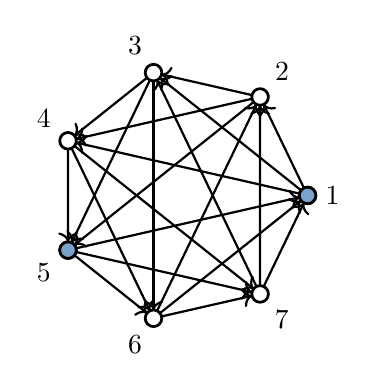
\begin{tikzpicture}[scale=0.8]
      \SetGraphUnit{2}
      \renewcommand*{\VertexLineColor}{black}
      \renewcommand*{\VertexLightFillColor}{white}
      \renewcommand*{\VertexSmallMinSize}{6pt}
      \renewcommand*{\VertexLineWidth}{1pt}
      %\SetVertexNoLabel
      \GraphInit[vstyle=Welsh]
      \Vertices{circle}{1,2,3,4,5,6,7} % the ... syntax doesn't work here
      \AddVertexColor{myblue}{1,5}

      \SetUpEdge[style={->,thick},color=black]
      \foreach \i in {1,...,7}
      { 
        \foreach
        [evaluate=\j as \k using {ifthenelse(Mod(\i+\j,7)==0,int(\i+\j),int(Mod(\i+\j,7)))}]
        \j in {1,2,3}
        { 
        \Edge(\i)(\k)
          }
        }

    \end{tikzpicture}
\end{frame}
\end{document}
